\section{Proposed Method: \method}\label{sec:proposal}

The proposed method \method organizes the generation of a preliminary sewer network into three moments:
data preparation, graph processing, and serialization of the resulting network.
The process starts from an urban area selected by the user, from which the system obtains public street data, enriches vertices with elevation, builds an editable graph, and allows manual adjustments before processing.


\subsection{Data preparation}

During data preparation, urban streets are obtained from OpenStreetMap through queries to the Overpass API and represented as GeoJSON \cite{osm2026}.
Topography is obtained through the OpenTopography API, which returns digital elevation models in GeoTIFF format \cite{opentopography2026}.
The system samples elevation values at street vertices, handles missing values or border artifacts, and keeps elevation attributes associated with graph nodes.
This step transforms raw geographic data into a structure that can be manipulated by the editor and by the backend.
Figure~\ref{fig:area-selection} illustrates the first interaction of this flow, in which the user defines a bounding box over the map and the system checks the selected area before fetching geospatial data.

\begin{figure}[ht]
\centering
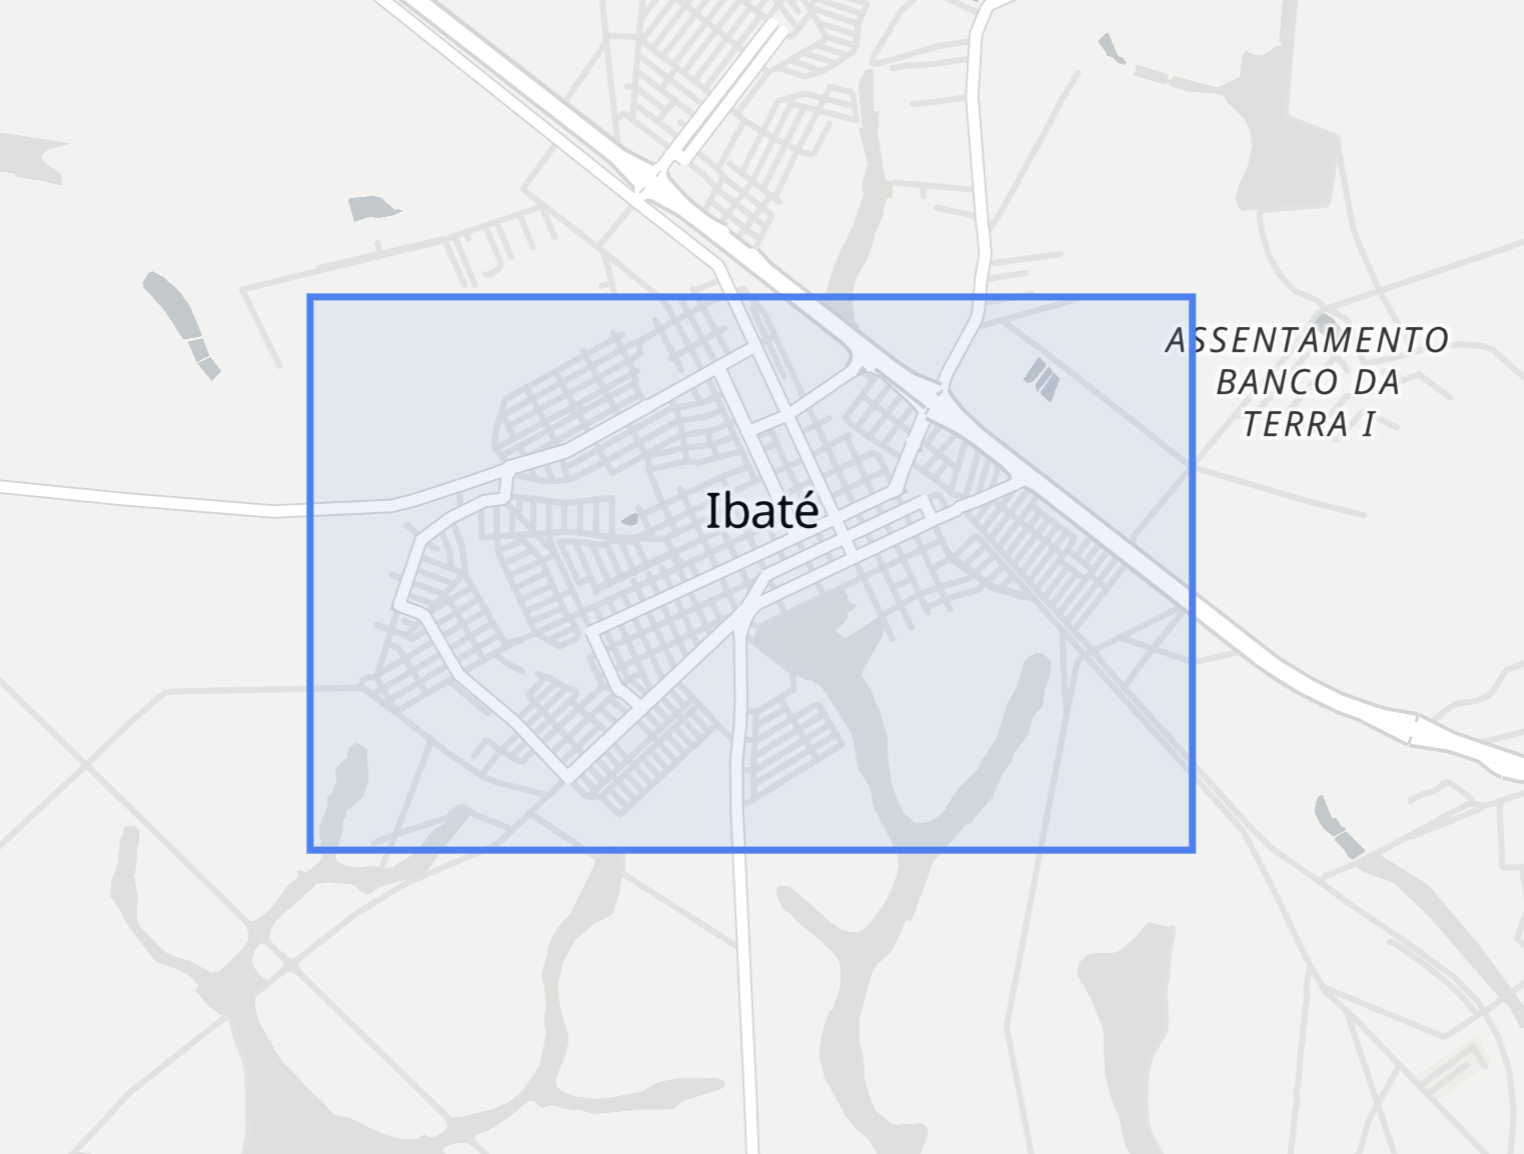
\includegraphics[trim={0 2cm 0 2cm},clip,width=.6\linewidth]{images/bounding-box-draw-zoom.png}
\caption{Area-selection step used to define the region processed by \method.}
\label{fig:area-selection}
\end{figure}


\subsection{Edited graph as processing input}

Before processing, the user can inspect and edit the graph.
This decision is methodologically important because the current system does not depend on an automatic reconstruction from the original GeoJSON after the user has made changes.
The edited graph becomes the ground truth for the pipeline.
In this way, the backend processes exactly the structure that the user visualized and adjusted, reducing the possibility of divergence between the interface and the computed network.
Figure~\ref{fig:graph-views} shows two complementary editor views of the same project: one emphasizing road categories and another emphasizing elevation values sampled along the graph.

\begin{figure}[ht]
\centering
    \begin{minipage}{.49\linewidth}
    \centering
    
\includegraphics[width=\linewidth]{images/map-view-streets.png}
    \end{minipage}
    \hfill
    \begin{minipage}{.49\linewidth}
    \centering
    
\includegraphics[width=\linewidth]{images/map-view-elevation.png}
    \end{minipage}
\caption{Editable graph views: road-category visualization on the left and elevation visualization on the right.}
\label{fig:graph-views}
\end{figure}

\subsection{Graph processing pipeline}

Processing starts by reconstructing the graph using the NetworkX Python library.
Then, the system applies safeguards over elevation data, identifies mandatory nodes, marks direction changes, removes redundant nodes, and applies spacing rules between manholes.
It then detects local maxima and minima, identifies grade breaks, and selects collection points.
These steps prepare the graph for routing by preserving relevant elements of the mesh and reducing points that do not contribute to network interpretation.

Gravitational routing uses the Repeated Shortest Path Heuristic (RSPH) to connect mandatory nodes and collection points to an outlet or to local collectors.
The heuristic performs successive least-cost path searches, updates the network under construction, and favors the reuse of trunks.
After routing, the pipeline repairs missing edge coverage, removes cycles when necessary, optimizes the position and quantity of nodes, and assigns inspection accessories to the remaining physical nodes.
The output is a serialized preliminary network with nodes, edges, lengths, slopes, elevations, flow directions, and relevant point markers.
Figure~\ref{fig:rsph-routing} details the routed network after processing, including flow-direction arrows and collection-point markers used to inspect the generated solution.

\begin{figure}[ht]
\centering
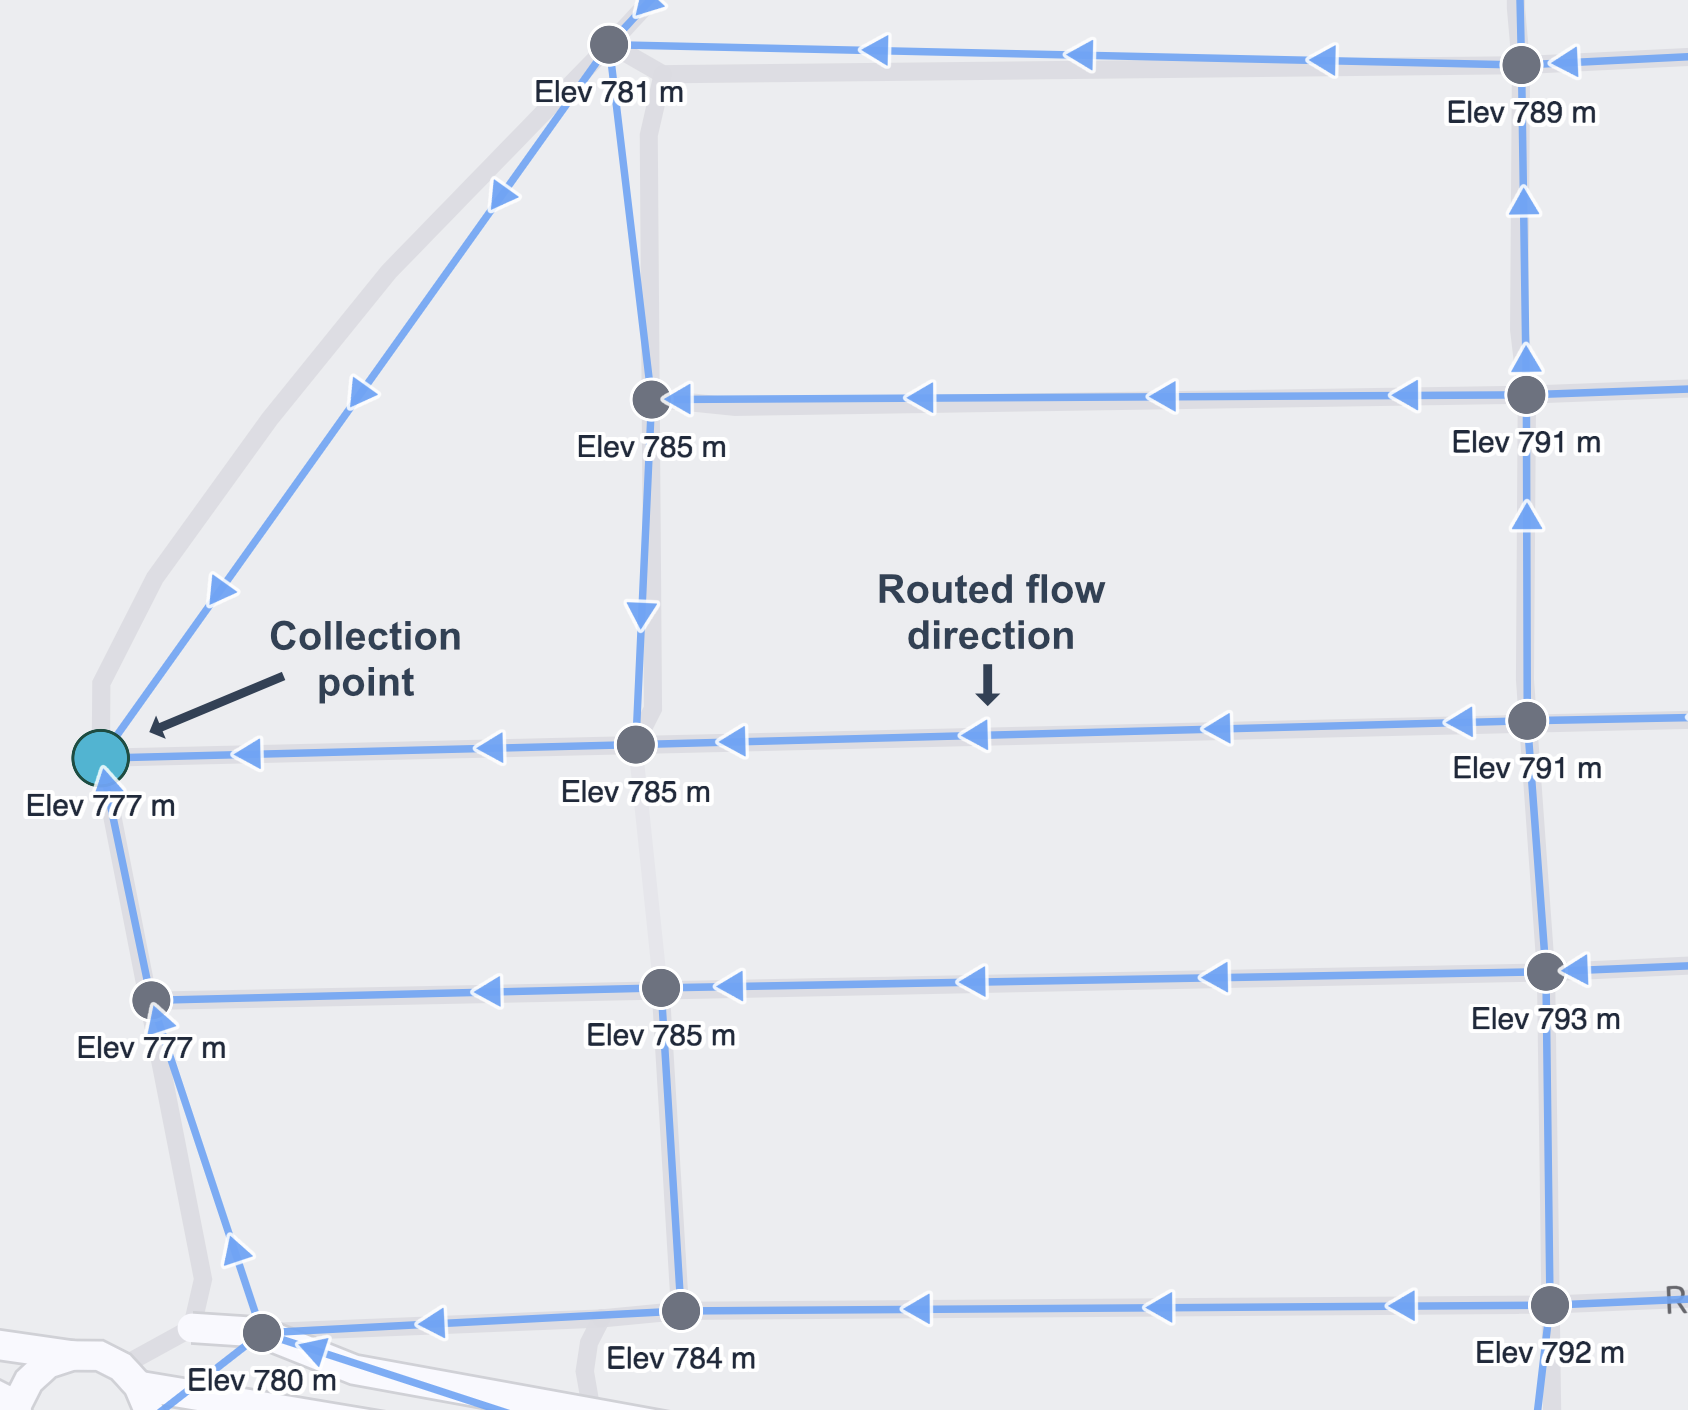
\includegraphics[trim={0 5cm 0 5cm},clip,width=.7\linewidth]{images/sewer-flow.png}
\caption{Detailed view of the processed network, highlighting RSPH routing, flow direction, sampled node elevations, and the selected collection point (in blue).}
\label{fig:rsph-routing}
\end{figure}

\subsection{Architecture and implementation}

The system is organized as a polyglot monorepo.
The JavaScript/TypeScript part uses a pnpm workspace, while the Python part uses a uv workspace.
This organization keeps related applications and packages in the same repository, separating responsibilities without duplicating domain concepts.
% 
The frontend was developed with Next.js, React, TypeScript, Tailwind CSS, MapLibre, React Map GL, Zustand, and React Query.
The interface includes map area selection, street import, interactive graph editing, visualization controls, editing state, result panels, and alternation between the original mesh and the processed network.
The editor supports node selection, movement, creation, connection, splitting, and removal, as well as undo and redo actions.
% 
The backend was developed in Python with FastAPI, Pydantic, SQLAlchemy, GeoAlchemy2, Shapely, Rasterio, NumPy, httpx, and NetworkX.
FastAPI exposes routes for project creation, listing, reading, and deletion, as well as routes for node extraction, elevation enrichment, and network processing.
NetworkX is used as the graph structure for algorithmic steps, while PostGIS provides geospatial persistence.

Projects are persisted in PostgreSQL with the PostGIS extension.
The database stores metadata, selected area, map center, statistics, street GeoJSON, and the processed network. Node and edge tables store spatial geometries and attributes such as elevation, node type, length, slope, and auxiliary properties.
In this way, the processed result can be saved, reloaded, and inspected later.
% 
Shared TypeScript packages were also created for geographic types, constants, and utilities, together with a Python package containing Pydantic types and geographic calculations.
This division follows the principle of sharing contracts, not implementations: each ecosystem keeps its own implementation, while the central concepts remain aligned through types, constants, and parity tests.


\subsection{Automatic building detection}

Sewage contribution estimates for each segment of the collector network depend, among other factors, on the type and density of the buildings served.
In traditional planning, this information is gathered manually or approximated by aggregate indicators, such as lot frontage length~\cite{rodrigues2020}.
To improve the accuracy of this estimate, URBANUS incorporates an automatic building detection module based on satellite imagery.

The module adopts deep learning approaches for semantic segmentation, automatically identifying the area occupied by buildings directly from medium- and high-resolution satellite images.
Techniques based on Convolutional Neural Networks (CNNs) and Vision Transformers (ViTs) have demonstrated strong performance on this task, extracting feature hierarchies that capture both local edge and texture details and long-range contextual relationships between image regions~\cite{alidoost2018cnn,dosovitskiy2021imageworth16x16words}.
The literature also points to hybrid architectures, such as CTCFNet and MMFFNet, that combine CNNs and Transformers to handle high inter-class similarity and variations in urban density~\cite{zhang2024building,zhou2024hierarchical}, representing promising directions for future work on this module.

In this work, two pre-trained models were experimentally evaluated with fine-tuning on the Massachusetts Buildings Dataset~\cite{MassachusettsBuildingsDataset}: SAM (\textit{Segment Anything Model}), a general-purpose segmentation model based on Transformers, and DeepLab~V3, a CNN-based model with dilated convolutions.

From an integration standpoint, the module exposes an API that receives the georeferenced area selected by the user and returns segmentation masks and the estimated built area per lot.
These data feed directly into the sewage contribution calculation in the URBANUS backend, allowing the collector network routing to be sensitive to the actual building density rather than relying on frontage-length estimates.

% A estimativa de contribuição de esgoto em cada trecho da rede coletora depende,
% entre outros fatores, do tipo e da densidade das edificações atendidas.
% No planejamento tradicional, essa informação é levantada manualmente ou
% aproximada por indicadores agregados, como o comprimento da testada dos lotes
% \cite{rodrigues2020}.
% Para aumentar a precisão dessa estimativa, o URBANUS incorpora um módulo de
% detecção automática de edificações a partir de imagens de satélite.


% O módulo adota abordagens de aprendizado profundo para segmentação semântica,
% identificando automaticamente a área ocupada por construções diretamente sobre
% imagens de média e alta resolução espacial.
% Técnicas baseadas em Redes Neurais Convolucionais (CNNs) e em Vision Transformers
% (ViTs) têm demonstrado desempenho expressivo nessa tarefa, extraindo hierarquias
% de características que capturam tanto detalhes locais de bordas e texturas quanto
% relações contextuais de longa distância entre regiões da imagem
% \cite{alidoost2018cnn,dosovitskiy2021imageworth16x16words}.
% A literatura também aponta arquiteturas híbridas -- como a CTCFNet e a MMFFNet --
% que combinam CNNs e Transformers para lidar com alta similaridade entre classes
% e variações de densidade urbana \cite{zhang2024building,zhou2024hierarchical},
% representando direções promissoras para trabalhos futuros do módulo.


% Neste trabalho, foram avaliados experimentalmente dois modelos pré-treinados
% com ajuste fino sobre o Massachusetts Buildings Dataset
% \cite{MassachusettsBuildingsDataset}: o SAM (\textit{Segment Anything Model}),
% modelo generalista de segmentação baseado em Transformers, e o DeepLab V3,
% modelo baseado em CNNs com convoluções dilatadas.
% A Tabela~\ref{tab:seg_results} compara os resultados de segmentação obtidos
% antes e após o ajuste fino de cada modelo.


% O ajuste fino produziu ganhos expressivos em ambos os modelos.
% O SAM elevou seu IoU médio de 0,160 para 0,586, e o DeepLab V3 passou de
% 0,177 para 0,600, com Dice médio de 0,747 -- valores que indicam segmentações
% suficientemente precisas para alimentar a estimativa de contribuição de esgoto
% no pipeline do URBANUS.

% \begin{figure}[ht]
%     \centering
%     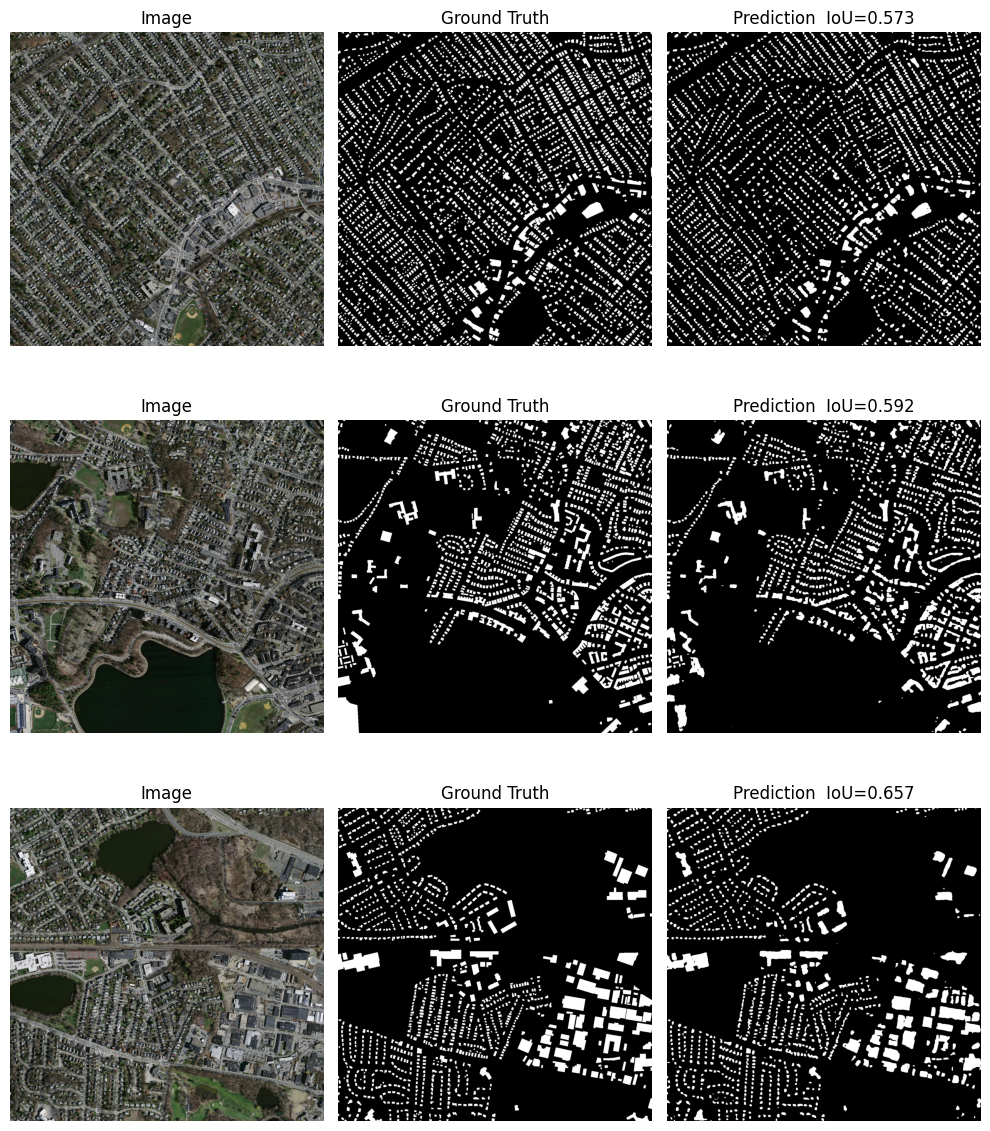
\includegraphics[width=0.9\textwidth]{images/DeeplabV3-finetuned_results.png}
%     \caption{Exemplos de segmentação de edificações pelo DeeplabV3 após ajuste fino sobre o Massachusetts Buildings Dataset. Cada linha apresenta, da esquerda para a direita: a imagem de satélite original, a máscara de referência (\textit{ground truth}) e a máscara predita pelo modelo}
%     \label{fig:DeeplabV3-results}
% \end{figure}

% É notável que o SAM, sendo um modelo generalista originalmente treinado para
% segmentação de propósito geral, tenha atingido desempenho comparável ao
% DeepLab V3 após o ajuste fino (Figuras~\ref{fig:SAM-finetuned-results}
% e), sugerindo boa capacidade de adaptação ao
% domínio de imagens de satélite.

% Como trabalho futuro, está prevista a contagem e classificação de instâncias
% individuais de edificações por lote, o que permitirá estimar a contribuição
% de esgoto com maior granularidade.
% Também serão investigadas arquiteturas híbridas CNN-Transformer e estratégias
% de fusão multimodal com modelos digitais de superfície (DSM), visando ampliar
% a acurácia em cenários de alta densidade urbana \cite{zhou2024hierarchical}.

% Do ponto de vista da integração com o restante da plataforma, o módulo expõe
% uma API que recebe a área georreferenciada selecionada pelo usuário e
% retorna as máscaras de segmentação e a área construída estimada por lote.
% Esses dados alimentam diretamente o cálculo de contribuição de esgoto no
% backend do URBANUS, permitindo que o roteamento da rede coletora seja
% sensível à densidade real das edificações em vez de depender de estimativas
% por comprimento de testada.
